% Plantilla IETAGRO Puerto Giraldo — 2° PARTE (2S)
% ==================================================
% Hoja de respuestas personalizada con QR.
% Datos del estudiante pre-impresos (no se escribe manualmente).
%
% Placeholders (rellenados por Python antes de compilar):
%   <<NOMBRE>>   Nombres y apellidos del estudiante (mayúsculas)
%   <<ID>>       Documento de identidad
%   <<CURSO>>    Curso (ej. 1101)
%   <<QR_PATH>>  Ruta absoluta del PNG del QR
%
% Diferencias con la plantilla 1S:
%   - Subtítulo: "SEGUNDA PARTE" en lugar de "PRIMERA PARTE"
%   - Etiqueta SESIÓN: "2° PARTE" en lugar de "1° PARTE"
%   - Columna 3 (P71-P105) tiene opciones A-H y es la más ancha (0.28w)
%   - Columna 4 (P106-P140) tiene opciones A-D y ancho normal (0.20w)

\documentclass[letterpaper]{article}
\usepackage[top=1.1cm, bottom=0.9cm, left=1.2cm, right=1.1cm]{geometry}
\usepackage{tikz}
\usepackage{graphicx}
\usetikzlibrary{calc, shapes.geometric, positioning}
\usepackage[T1]{fontenc}
\usepackage[utf8]{inputenc}
\usepackage{helvet}
\renewcommand{\familydefault}{\sfdefault}
\setlength{\parindent}{0pt}
\setlength{\parskip}{0pt}
\pagestyle{empty}

%================= AJUSTE FINO OMR =================
\newlength{\TMw}    \setlength{\TMw}{6pt}
\newlength{\Nw}     \setlength{\Nw}{14pt}
\newlength{\Bdia}   \setlength{\Bdia}{12pt}
\newlength{\Bsep}   \setlength{\Bsep}{1.5pt}
\newlength{\Brad}   \setlength{\Brad}{6pt}
\newlength{\Rowsep} \setlength{\Rowsep}{2pt}

\tikzset{cuadrocolumna/.style={
    draw, draw=black!70, line width=1.2pt,
    rounded corners=10pt, inner sep=8pt, outer sep=0pt,
    fill=white, align=left, anchor=north,
    text width=\linewidth-16pt
}}

\newcommand{\B}{%
  \makebox[\Bdia][c]{%
    \tikz[baseline=-2.8pt]{%
      \filldraw[fill=white, draw=black!70, line width=0.7pt, rounded corners=0pt, solid]
        (0,0) circle (\Brad);}%
  }%
}

\newcommand{\TM}{%
  \makebox[\TMw][c]{%
    \tikz[baseline=-4pt]{\fill[black, rounded corners=0pt, solid](0,-5pt) rectangle (\TMw,5pt);}%
  }%
}

\newcommand{\Q}[1]{%
  \noindent
  \TM\hspace{1pt}%
  \makebox[\Nw][r]{\scriptsize\textbf{#1.}}%
  \hspace{2pt}%
  \B\hspace{\Bsep}\B\hspace{\Bsep}\B\hspace{\Bsep}\B%
  \par\vspace{\Rowsep}%
}

\newcommand{\QH}[1]{%
  \noindent
  \TM\hspace{1pt}%
  \makebox[\Nw][r]{\scriptsize\textbf{#1.}}%
  \hspace{2pt}%
  \B\hspace{\Bsep}\B\hspace{\Bsep}\B\hspace{\Bsep}\B\hspace{\Bsep}%
  \B\hspace{\Bsep}\B\hspace{\Bsep}\B\hspace{\Bsep}\B%
  \par\vspace{\Rowsep}%
}

\newcommand{\HDR}{%
  \noindent
  \hspace{\TMw}\hspace{1pt}\hspace{\Nw}\hspace{2pt}%
  \foreach \L in {A,B,C,D}{%
    \makebox[\Bdia][c]{\footnotesize\textbf{\L}}\hspace{\Bsep}%
  }%
  \par\vspace{2pt}%
}

\newcommand{\HDRH}{%
  \noindent
  \hspace{\TMw}\hspace{1pt}\hspace{\Nw}\hspace{2pt}%
  \foreach \L in {A,B,C,D,E,F,G,H}{%
    \makebox[\Bdia][c]{\footnotesize\textbf{\L}}\hspace{\Bsep}%
  }%
  \par\vspace{2pt}%
}

\begin{document}

%================= MARCADORES DE PÁGINA =================
\begin{tikzpicture}[remember picture, overlay]
  \fill[black] ($(current page.north west)+(8mm,-8mm)$)  rectangle ++(8mm,-8mm);
  \fill[black] ($(current page.north east)+(-8mm,-8mm)$) rectangle ++(-8mm,-8mm);
  \fill[black] ($(current page.south west)+(8mm,16mm)$)  rectangle ++(8mm,8mm);
  \fill[black] ($(current page.south east)+(-8mm,16mm)$) rectangle ++(-8mm,8mm);
\end{tikzpicture}

\vspace*{2mm}

% ================== ENCABEZADO IETAGRO (REDISEÑADO) ==================
\noindent\makebox[\textwidth][c]{
\begin{tikzpicture}[x=1cm, y=1cm]

% --- Caja principal (4 cm de alto) ---
\draw[line width=2pt, rounded corners=10pt] (-9, -2.1) rectangle (9, -6.1);

% --- Franja vertical izquierda (acento visual) ---
\fill[black!85, rounded corners=10pt] (-9, -2.1) rectangle (-8.55, -6.1);
\fill[black!85] (-8.85, -2.1) rectangle (-8.55, -6.1);

% --- Título principal ---
\node[font=\Large\bfseries, anchor=west] at (-8.3, -2.65)
  {IETAGRO PUERTO GIRALDO};

% --- Subtítulo ---
\node[font=\normalsize, text=black!60, anchor=west] at (-8.3, -3.20)
  {Simulacro Saber 11°  ·  SEGUNDA PARTE};

% --- Línea fina separadora ---
\draw[line width=0.8pt, black!30] (-8.3, -3.55) -- (4.5, -3.55);

% --- Estudiante ---
\node[font=\scriptsize\bfseries, text=black!50, anchor=west] at (-8.3, -3.95)
  {ESTUDIANTE};
\node[font=\large\bfseries, anchor=west] at (-8.3, -4.45)
  {<<NOMBRE>>};

% --- Datos inferiores ---
\node[font=\scriptsize\bfseries, text=black!50, anchor=west] at (-8.3, -5.10)
  {DOCUMENTO};
\node[font=\large\bfseries, anchor=west] at (-8.3, -5.55)
  {<<ID>>};

\node[font=\scriptsize\bfseries, text=black!50, anchor=west] at (-3.8, -5.10)
  {CURSO};
\node[font=\large\bfseries, anchor=west] at (-3.8, -5.55)
  {<<CURSO>>};

\node[font=\scriptsize\bfseries, text=black!50, anchor=west] at (-1.0, -5.10)
  {SESIÓN};
\node[font=\large\bfseries, anchor=west] at (-1.0, -5.55)
  {2° PARTE};

% --- QR (32mm × 32mm) ---
\node[anchor=center] at (6.9, -4.10) {%
  \includegraphics[width=3.2cm]{<<QR_PATH>>}};

\end{tikzpicture}
}

\vspace{6mm}

%================= RESPUESTAS (2° PARTE — columna 3 con A-H) =================
\noindent
\begin{minipage}[t]{0.20\textwidth}
  \vspace{0pt}
  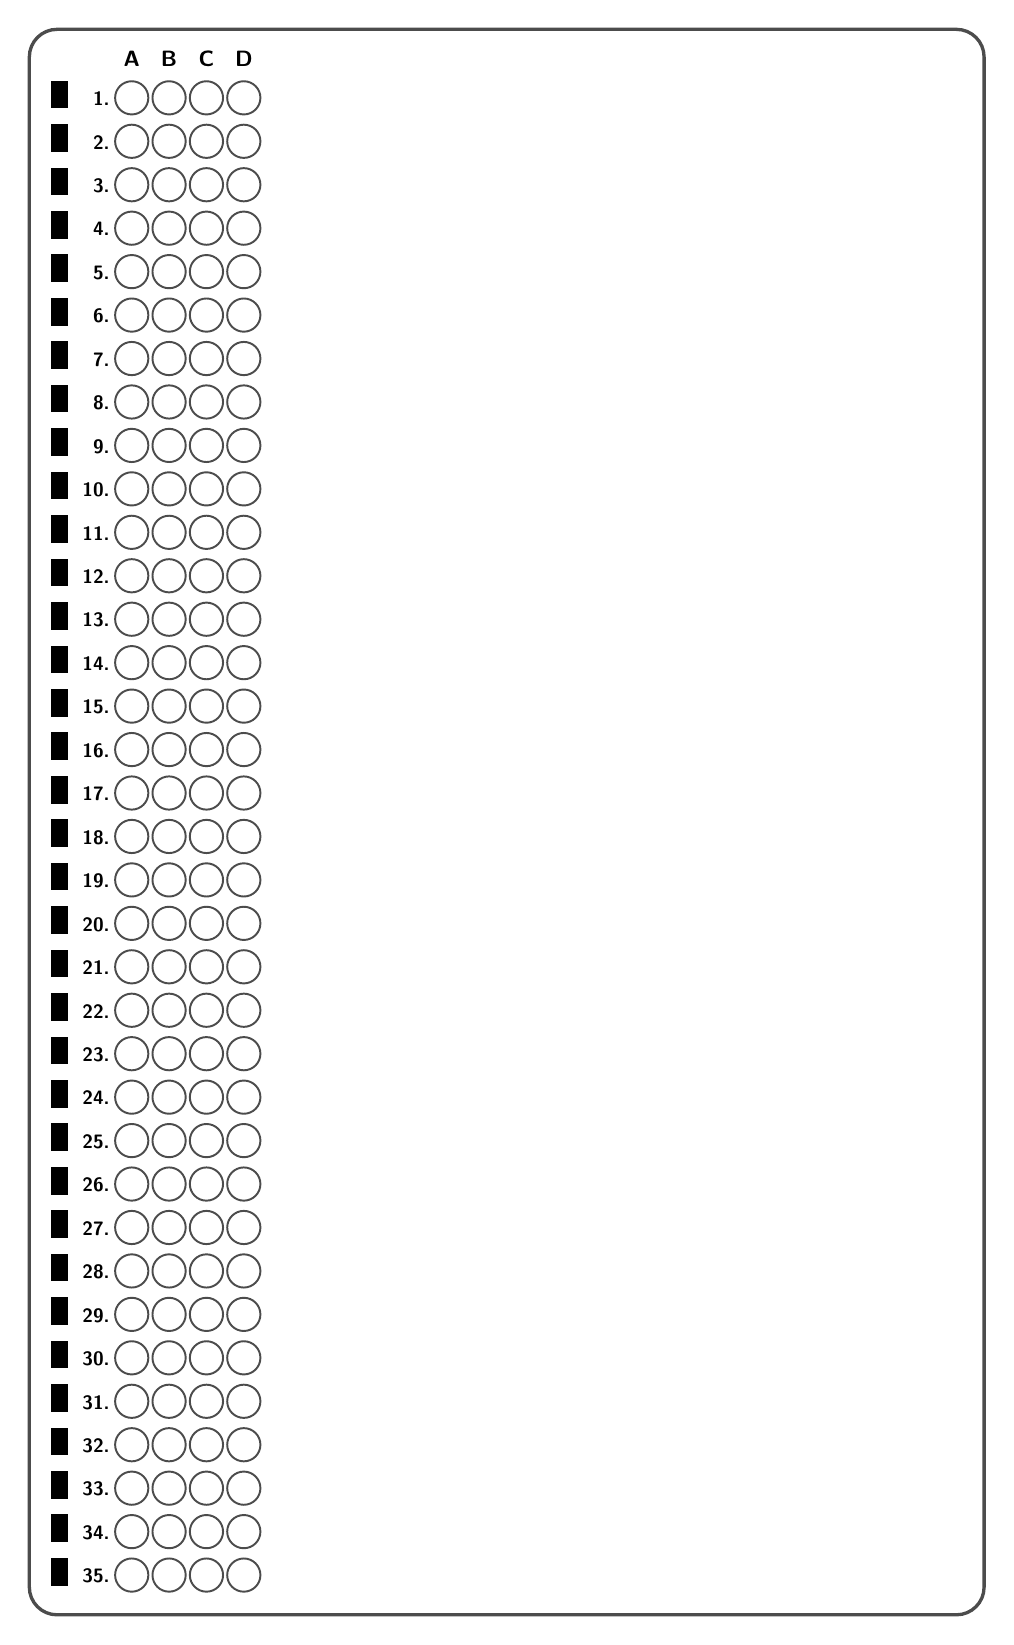
\begin{tikzpicture}
    \node[cuadrocolumna] { \HDR \foreach \n in {1,...,35}{\Q{\n}} };
  \end{tikzpicture}
\end{minipage}%
\hfill
\begin{minipage}[t]{0.20\textwidth}
  \vspace{0pt}
  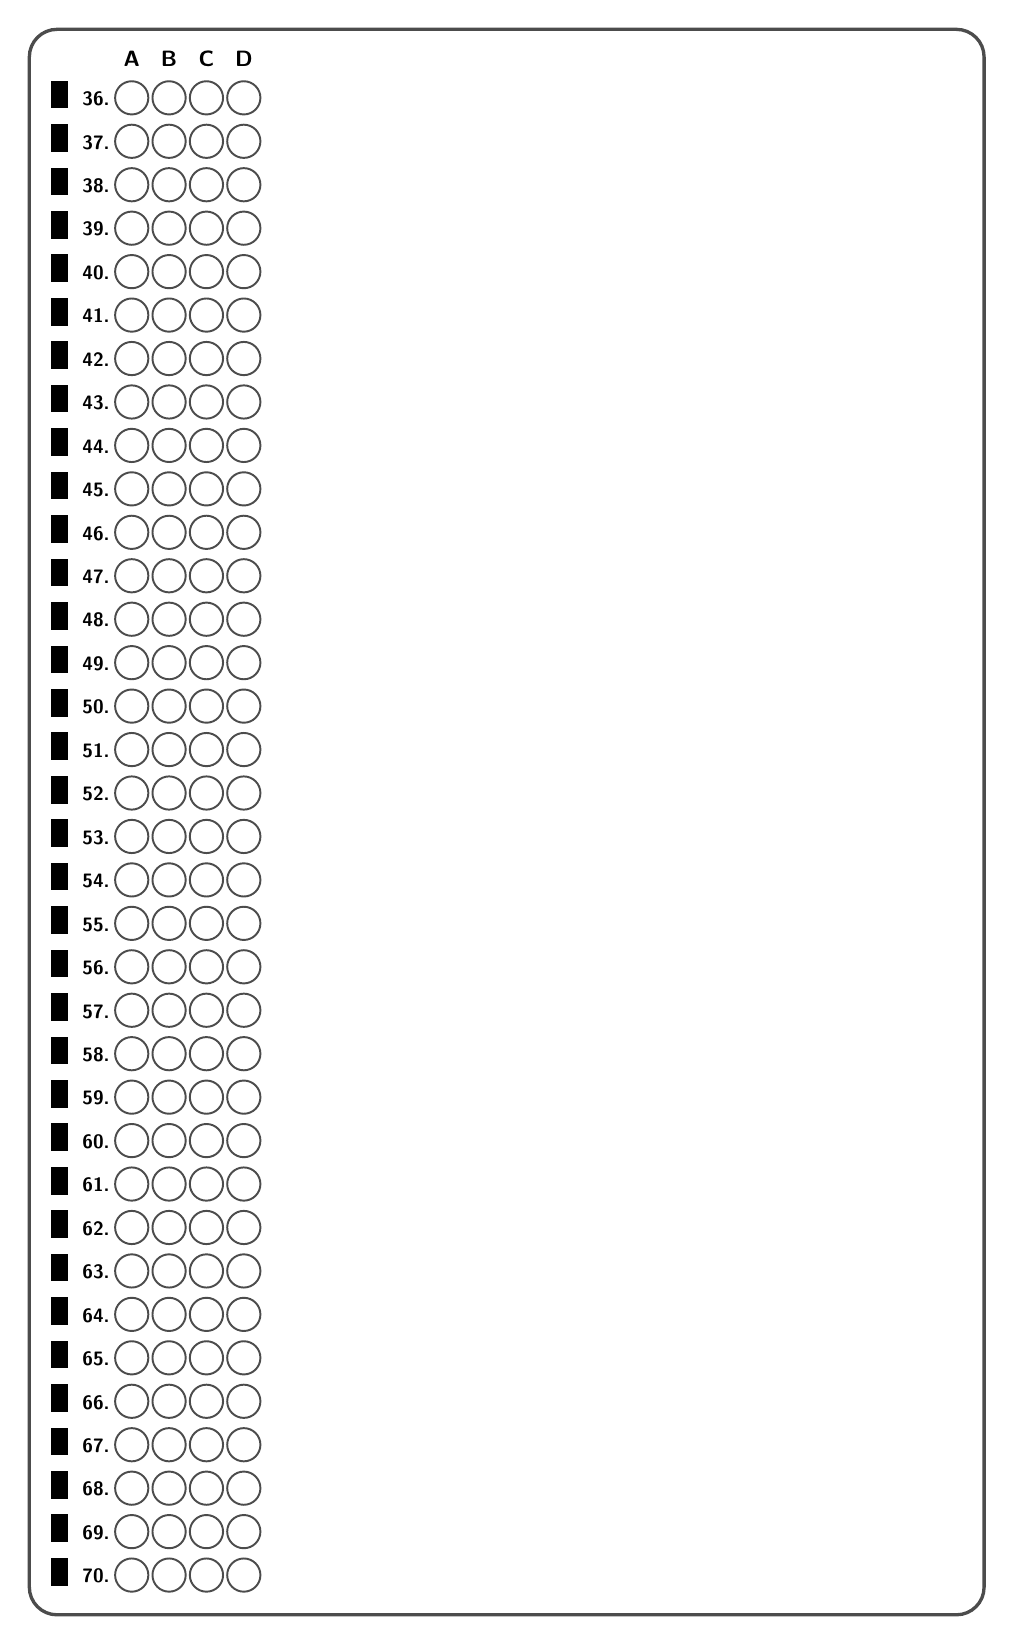
\begin{tikzpicture}
    \node[cuadrocolumna] { \HDR \foreach \n in {36,...,70}{\Q{\n}} };
  \end{tikzpicture}
\end{minipage}%
\hfill
\begin{minipage}[t]{0.28\textwidth}
  \vspace{0pt}
  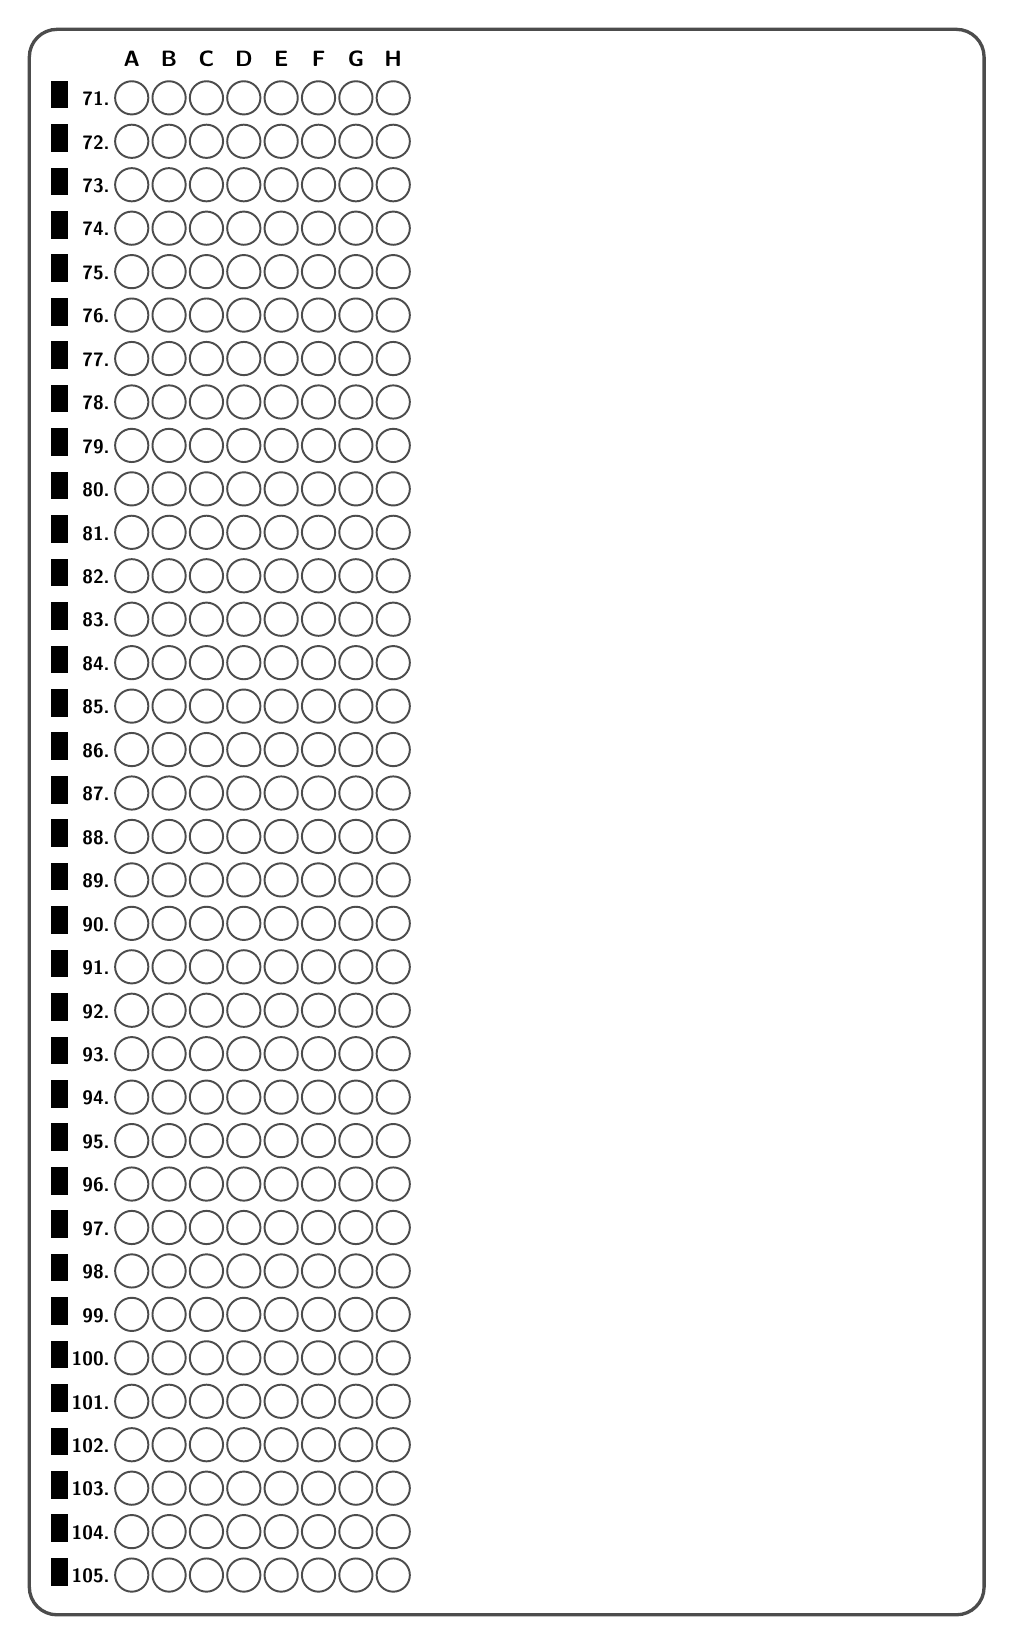
\begin{tikzpicture}
    \node[cuadrocolumna] { \HDRH \foreach \n in {71,...,105}{\QH{\n}} };
  \end{tikzpicture}
\end{minipage}%
\hfill
\begin{minipage}[t]{0.20\textwidth}
  \vspace{0pt}
  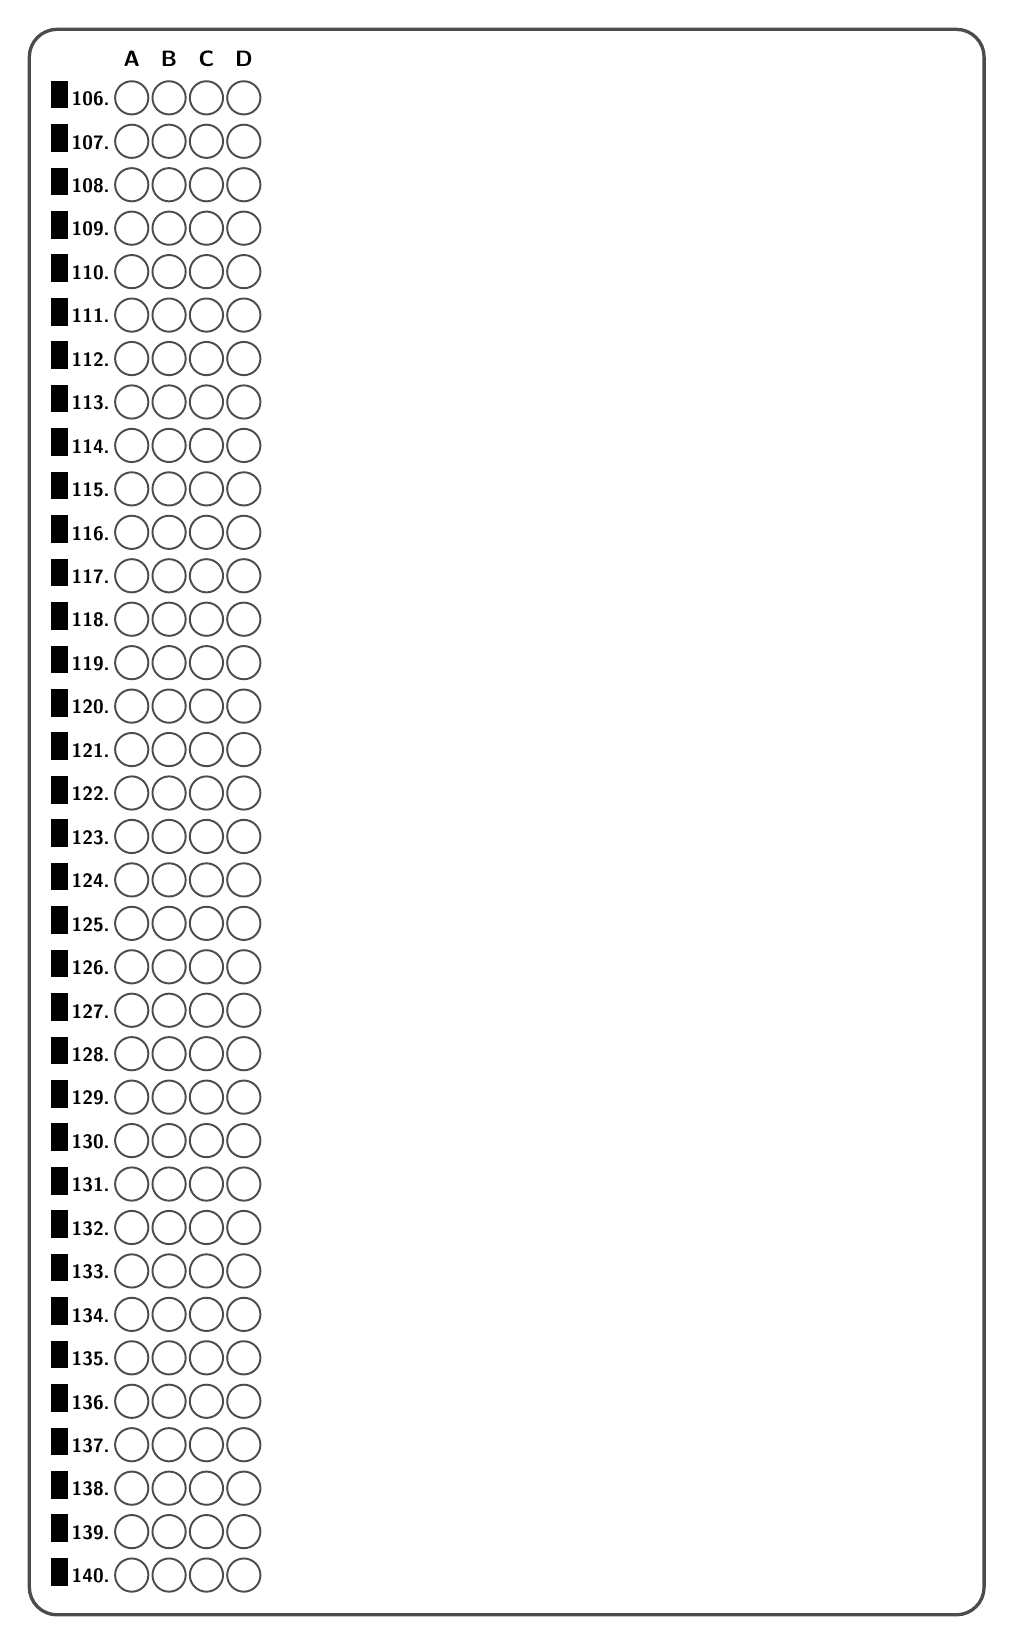
\begin{tikzpicture}
    \node[cuadrocolumna] { \HDR \foreach \n in {106,...,140}{\Q{\n}} };
  \end{tikzpicture}
\end{minipage}

\end{document}

